
\section{Multi-Layer Perceptron}

Next, the \texttt{neuralnet} package \cite{neuralnet} is used to fit a multi-layer perceptron network to the training data.  Several networks were tested, containing one hidden layer of differing sizes.  For computational efficiency and for simplicity, deeper networks were not considered.  The function uses resilient backpropagation by default and sigmoid activation between layers.  A diagram of the network is displayed below:

\begin{figure}[H]
    \center
    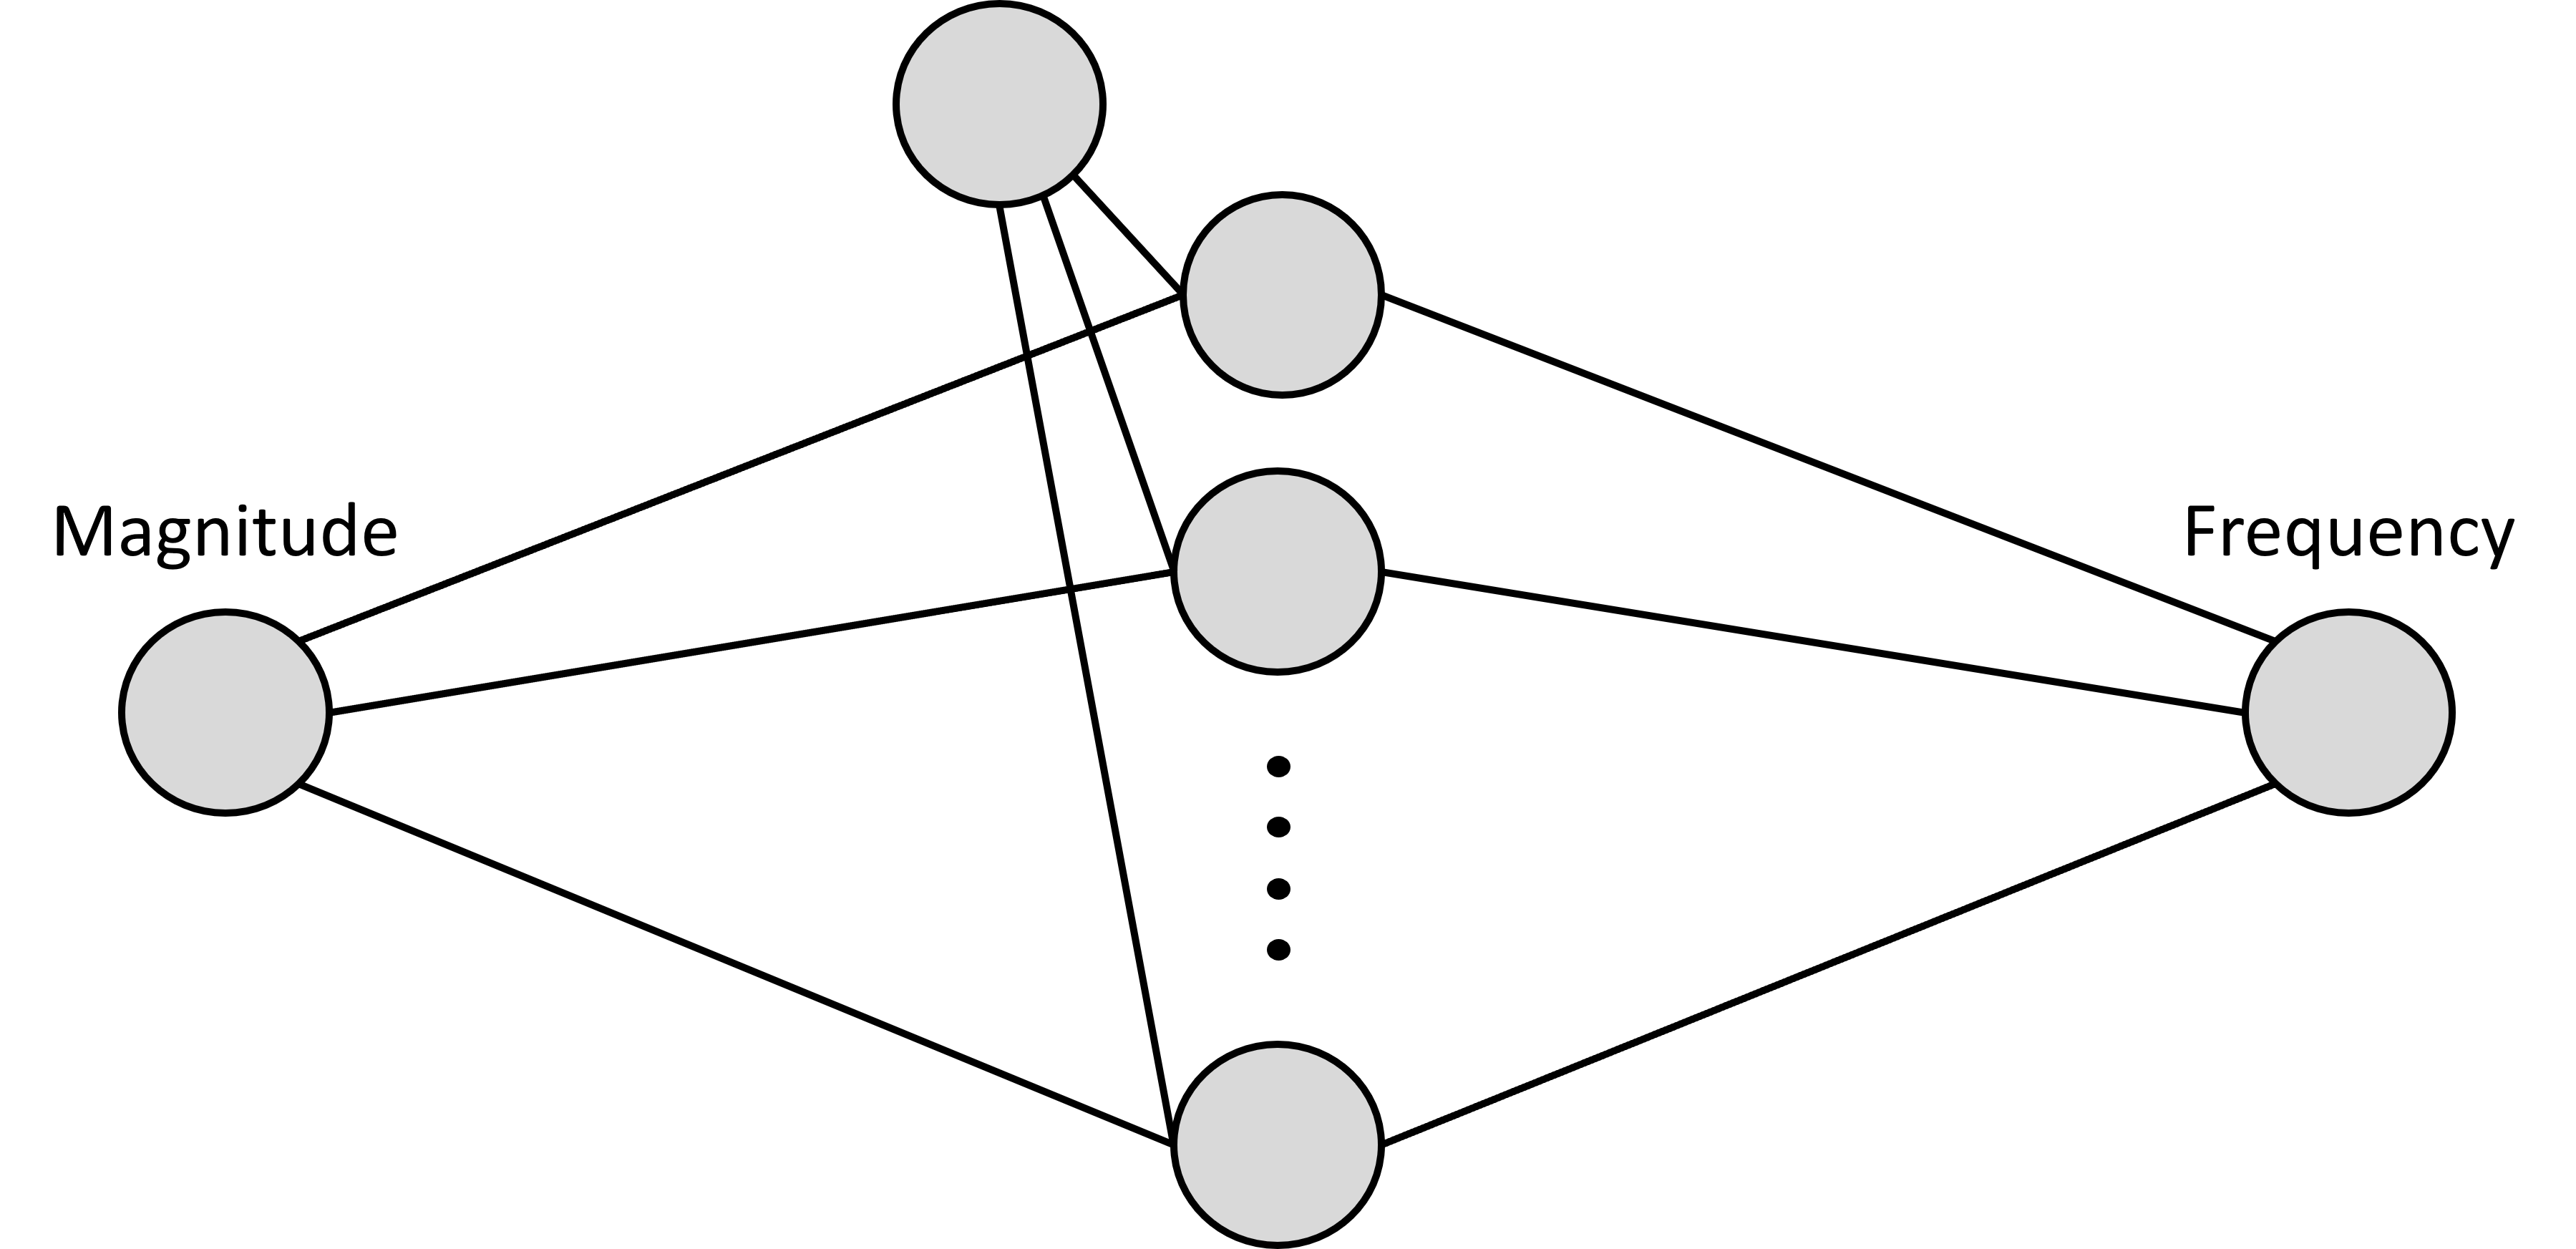
\includegraphics[width=0.55\linewidth]{Figures/MLPdiag.png}
   % \vspace{-10pt}
    \caption{\footnotesize{Two-layer MLP network(s) of various sizes, with weight and bias connections displayed.  Magnitude is the explanatory variable and Frequency is the response.  Sigmoid is the hidden layer activation.}}
    \label{tohoku_unfit}
\end{figure}

To obtain a more accurate test error, cross-validation was applied to aggregate the baseline test error from 200 Poisson regression models. Because the data was so sparse, the distribution of calculated test errors was very wide and contained a few outliers that skewed the resulting average.  Thus, the \textit{median} test error was taken to better measure prediction accuracy.  To determine the optimal number of neurons in the hidden layer, 50 of each network was generated and the median test error calculated.  It was hoped to compare as many of each neural network as the Poisson model, but in order to save computation this number had to reduced.

% latex table generated in R 4.2.2 by xtable 1.8-4 package
% Wed May  3 23:45:14 2023
\begin{table}[H]
\centering
\begin{tabular}{rlr}
  \hline
 Baseline & Test Error \\ 
  \hline
  Poisson Regression Model & 0.1862851 \\ 
  \hline
 Hidden Units & Test Error \\ 
  \hline
3 & 0.2441865 \\ 
  6 & 0.2818492 \\ 
  9 & 0.1785652 \\ 
  10 & 0.2633863 \\ 
  20 & 0.1706793 \\ 
   \hline
\end{tabular}
   \caption{\footnotesize Test accuracy for a two-layer multi-layer perceptron network of different hidden layer sizes compared to the baseline Poisson model.}
\end{table}


Based on these results, it is recommended to choose a simpler model: the Poisson regression has a comparable Test Error to the MLP for any size surveyed.  It even out performs the MLP in most cases.  By choosing a simpler model, the Poisson model would be able to extrapolate results better than any MLP surveyed here devoid of regularization.

Additionally, the cost function used in the MLP model is not appropriate for the task.  By default, the \texttt{neuralnet} package uses the least squares criterion; essentially treating the model like a linear regression task.  In fact, the data had to be transformed to the logarithmic scale in order for the resilient backpropagation algorithm to converge for most cases.  Several attempts were made to replicate the networks used in a simulation study by (Fallah,et.al, 2009 \cite{fallah2009nonlinear}) to compare the performance of a neural network Poisson regression model with its traditional counterpart.  Such a model would have to be amended to compete with a cost function for count data.  Particularly, based on negative log likelihood for Poisson regression, the cost function would be:
$$
E_D = - \sum_{i=1}^N \left[ -\hat{y_i} + y_i log(\hat{y_i}) \right]
$$

The final result would be exponentiated to generate predictions.
However no successful attempt was made using the \texttt{neuralnet} package, and instead a linear regression MLP was used. (See Appendix for more details)
